
\begin{quote}
Numbers generated by \texttt{eval/downstream.py} and, for \S5.7, by \texttt{eval/score\_planner.py}; reproducible from \texttt{outputs/rq2\_report.json} and \texttt{outputs/planner\_scores.json}.
\end{quote}

This chapter answers RQ2 with a controlled experiment over three label sources. Section 5.1 states the design, \S5.2 the result, \S5.3 examines why self-training fails to rescue the human labels, \S5.4 the mechanism and its consistency checks, \S5.5 the boundaries of the claim, and \S5.6 the connection to the source paper's robot-planning chain. Section 5.7 then tests that chain one link further, asking whether the label source changes the plan an LLM planner produces for a robot, and \S5.8 gives the answer.

\section{The controlled experiment}

RQ2 asks whether the automatic labels are good enough to \textit{train} a relation model as effectively as human labels. The experiment isolates exactly that variable: one lightweight classifier per predicate (a small MLP over pure geometric pair features: relative position, depth difference, box geometry, size-relative gap, mask-contact fractions), trained with \textbf{identical features, architecture, seed, positive-oversampling and group split}, then evaluated against the \textbf{held-out human gold} (annotator groups 6--8, whose data influenced no threshold, no calibration, and no training). The only difference between the runs is the supervision source. (Training uses a fixed 60-iteration budget for every classifier; some do not fully converge, identically for every source; the comparison is between supervision signals under equal compute, not between tuned models.)

Three sources are compared, because two would leave the obvious objection unanswered.

\begin{itemize}
\item \textbf{Human.} The \textasciitilde{}10\% of ordered pairs the annotators chose to label.
\item \textbf{Automatic.} Every pair the tool's rules fire on: dense and
rule-consistent.
\item \textbf{Self-trained (pseudo-labelled).} The rival remedy from the
semi-supervised literature (\S2.4), implemented rather than argued about. A teacher is trained on the human labels exactly as in the human arm; it then predicts the \textit{unannotated} training pairs, its confident predictions (probability $\geq$ 0.90 either way) become pseudo-labels, and a student is retrained on the union of real and pseudo labels (Lee, 2013). A pair the annotators touched at all counts as labelled, since their silence on its other predicates is informative; a pair they never recorded is the unlabelled pool. This arm answers the question a reader should ask before accepting the project's premise: if the human labels are too sparse, why not simply stretch them?
\end{itemize}

Each source labels the same pairs its own way, and each model inherits its source's character. That contrast is the experiment.

\section{Result}

Averaged over three seeds (42/43/44); each cell shows mean (min--max):

\begin{center}
\small
\begin{longtable}{lrrrr}
\caption{Downstream recall against held-out human gold for the three label sources.}\\
\hline
predicate & human-trained & self-trained & auto-trained & gold (held-out) \\
\hline
\endfirsthead
\hline
predicate & human-trained & self-trained & auto-trained & gold (held-out) \\
\hline
\endhead
on & 0.84 (0.83--0.86) & 0.90 (0.89--0.92) & 0.92 (0.92--0.93) & 348 \\
under & 0.44 (0.36--0.53) & 0.59 (0.59--0.60) & 0.92 (0.92--0.93) & 192 \\
to the left of & 0.22 (0.18--0.29) & 0.31 (0.27--0.34) & 0.95 (0.95--0.95) & 446 \\
to the right of & 0.25 (0.22--0.31) & 0.38 (0.37--0.39) & 0.99 (0.99--0.99) & 550 \\
in front of & 0.09 (0.08--0.10) & 0.12 (0.12--0.13) & 0.19 (0.19--0.19) & 609 \\
behind & 0.15 (0.12--0.17) & 0.22 (0.17--0.28) & 0.33 (0.32--0.34) & 580 \\
near & 0.08 (0.00--0.19) & 0.03 (0.00--0.06) & 1.00 (1.00--1.00) & 93 \\
\textbf{mean} & \textbf{0.30} & \textbf{0.36} & \textbf{0.76} &  \\
\hline
\end{longtable}
\end{center}

Training on the automatic labels multiplies downstream mean recall by \textasciitilde{}2.5 against the human annotators' own held-out labels: 0.76 vs 0.30. Self-training lands between the two but far closer to the floor: it improves the human baseline on six of seven predicates and lifts the mean to 0.36, which closes \textbf{15\% of the distance} between the human and automatic arms. Stretching the existing labels helps; it does not substitute for labelling every pair consistently.

The seed spreads carry a second result. The auto-trained model's recall varies by at most 0.02 across seeds on every predicate, while the human-trained model's varies by up to 0.19 (\texttt{near} spans 0.00--0.19) and the self-trained model inherits that instability (\texttt{behind} spans 0.17--0.28). Sparse supervision is not just weaker, it is \textit{unstable}, its outcome hostage to sampling noise, and self-training passes the instability on to its student.

\begin{figure}[htbp]
\centering
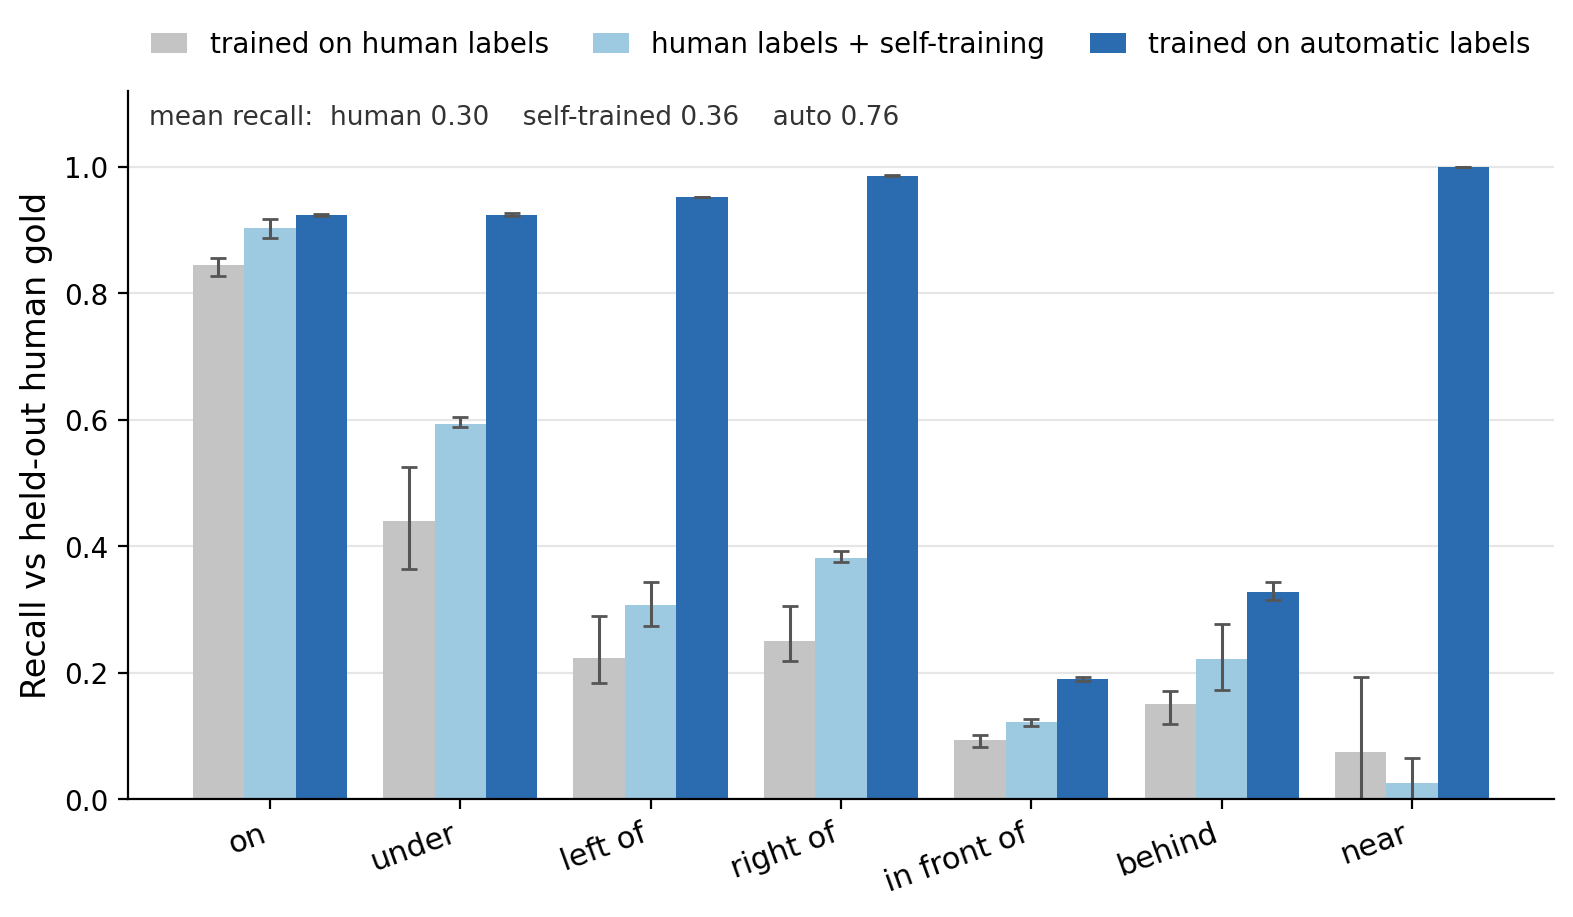
\includegraphics[width=0.95\textwidth]{figures/rq2-comparison.png}
\caption{Downstream recall against held-out human gold for the three label sources. Self-training improves on the human labels everywhere except \texttt{near}, where it falls below them.}
\label{fig:rq2-comparison}
\end{figure}

\section{Why self-training does not rescue the human labels}

The pseudo-label arm's own bookkeeping explains its ceiling precisely. Of the 60,762 training pairs, the annotators recorded just \textbf{6,026}. Filling in the rest, the teacher adds roughly \textbf{54,000 confident negative} pseudo-labels per predicate against only \textbf{36 to 67 confident positives}: a ratio of about 1,000 to 1. The teacher, trained on annotation in which most pairs carry no label, has learned above all that pairs usually have no relation, and self-training feeds that conviction back to the student as though it were evidence. What propagates is not the annotators' knowledge but their silence.

This is the failure mode \S2.4 predicted from the literature, now measured. Pseudo-labelling is well behaved when the labelled seed is a representative sample of the unlabelled pool. Here it is neither representative nor complete: the annotators labelled the pairs they found salient, so absence of a label conflates "no relation holds" with "nobody looked". A student trained on the union cannot distinguish the two, and inherits a systematic bias towards silence.

The \texttt{near} row makes the point sharply. Human-trained recall is already near-collapse at 0.08, and self-training pushes it \textit{down} to 0.03. Only three of nine annotator groups used the label at all, so the teacher's notion of "near" is both weak and idiosyncratic; its confident pseudo-labels then bury what little positive signal existed. Where the seed is defective, self-training does not merely fail to help, it can actively amplify the defect. The automatic labels reach 1.00 on the same evaluation, because the fitted threshold applies one definition to every pair rather than extrapolating three annotators' habits.

The comparison is therefore not "programmatic labels beat doing nothing", but "programmatic labels beat the standard remedy, under identical conditions, closing more than six times as much of the available gap". Active learning is not tested here because it fails for a different and simpler reason: it still buys human labels, so it lowers the bottleneck's cost without removing it, and it has no mechanism at all for the inconsistency between annotators that Chapter 4 measures.

\section{Why the automatic labels win, and two consistency checks}

The mechanism is the one this dissertation measures throughout: the human labels are \textit{sparse} (\textasciitilde{}10\% of pairs) and \textit{inconsistent} (three of nine annotators used \texttt{near}; two inverted the front/behind convention; support was often labelled in one direction only). A classifier trained on sparse, inconsistent supervision learns above all to be silent; its recall collapses exactly where human labelling was thinnest (\texttt{near} 0.08, lateral 0.22--0.25). The automatic labels are dense and rule-consistent, so the same model actually learns the geometry (near 1.00, lateral 0.95--0.99, support 0.92). This is the weak-supervision prediction (\S2.3) confirmed under controlled conditions: dense, consistent programmatic labels out-teach scarce gold labels when supervision, not model capacity, is the bottleneck.

Two checks argue the result is real rather than an artefact. First, the auto-trained model's profile almost exactly reproduces the rule layer's own held-out performance (mean 0.76; front/behind 0.19/0.33 $\approx$ the rules' held-out 0.20/0.35): the classifier \textit{distilled the annotator}, which is precisely what "the labels are learnable" means. Second, all three arms face identical conditions everywhere: the same features, the same oversampling cap, the same held-out gold including the convention-inverted annotators, which penalises every arm's front/behind equally.

\section{Honest boundaries}

The evaluation gold is itself sparse human annotation, so recall (not precision) is the reported metric, mirroring the RQ1 protocol. The human-trained model's weakness is partly a property of \textit{any} sparse supervision at this scale; with many more human labels it would improve, but producing many more human labels is exactly the bottleneck this project removes, and the self-trained arm shows the shortfall cannot simply be computed away. The front/behind rows are depressed for every arm by the held-out groups' inverted convention (Chapter 4); the comparison between sources remains fair because the penalty is shared.

One structural caveat deserves stating plainly. The classifier's features are geometric, and the automatic labels were generated by rules over closely related geometry, so the auto-trained arm's task is partly to re-learn its own generator; read alone, this chapter shows the automatic labels are \textit{learnable} and the human labels are not, rather than that automatic labels win under any featurisation. Three things keep the comparison meaningful: every arm receives the identical features, so the featurisation advantages no source; "the labels are learnable" is itself the property RQ2 asks about, since a downstream consumer must extract a consistent signal from the labels; and Chapter 6 removes the circularity entirely by repeating the comparison in a full scene-graph model with visual features, where the density and consistency effects persist in the training dynamics and the zero-shot generalisation even though the headline verdict changes.

\section{From labels to robots: where this sits in the source paper's chain}

The source paper's end goal is explicit: spatial understanding exists so that robots can plan. Their motivating example shows an LLM planner failing to remove a cube before grasping the book beneath it until SGG-derived relations are supplied, after which it "generates executable, spatially-aware plans." The paper's own evaluation of that chain stops at SGG quality: six models benchmarked on the human labels, topping out at mR@100 = 0.49 (VCTree), with every model saturating by epoch 2--6 and \texttt{near} stuck at 0.22--0.25 (\S2.2).

Each of those benchmark symptoms has a cause this dissertation measured and a remedy it built. Saturation within six epochs is what training on 9,313 sparse triplets looks like; the automatic labels provide 20$\times$ the supervision on the same images. The universal \texttt{near} failure is what training on an undefined, three-annotator label looks like; the fitted-threshold labels are perfectly learnable (this chapter's proxy reaches 1.00). And the depth predicates were being actively taught two opposite conventions by different annotators; the automatic labels apply one. The controlled experiment above is the proxy for the SGG step of the chain, and it measures the effect as large. The direct test, training the paper's own benchmark model on automatic versus human labels and comparing mR@100, is executed in Chapter 6. Three concrete predictions are registered here, before that run: later saturation, a higher plateau, and the recovery of \texttt{near}. Chapter 6 judges all three.

\section{The planner experiment: does the label source change what a robot would do?}

Section 5.6 ends with the source paper's motivating example, in which an LLM planner fails to remove a cube before grasping the book beneath it until spatial relations are supplied. That example is an assertion in the paper, illustrated on one scene. It can be run as an experiment, and this section runs it.

\textbf{Design.} Twenty-five held-out scenes were selected in which a target object has a second object physically resting on it, so any safe plan must move the occluder first. Each scene is put to an LLM planner (\texttt{gemini-flash-latest}) three times, in prompts differing only in what they state about the scene: \textbf{A} lists the objects and nothing else, \textbf{B} adds the human-annotated relationships, \textbf{C} adds the automatically computed ones. The task sentence, the object list and the instruction to give a minimal numbered plan are identical across conditions. All three conditions of a scene are answered by one model in one sitting, so no scene can be split across models by a quota interruption (\texttt{scripts/run\_planner\_llm.py}).

\textbf{Scoring.} A plan is safe if it moves the occluding object in an earlier step than the one that grasps the target. Judgements are made by published rules rather than by reading (\texttt{eval/score\_planner.py}), for two reasons: the rules never see the condition, so scoring is blind by construction, which matters when the author has a stake in the result; and a reader who disputes a verdict can inspect the rule instead of trusting a judgement. The rules were checked against a hand-read sample, which is the only thing that makes them trustworthy and which caught a real defect: models frequently open with a preamble restating the task ("To pick up box0 safely, follow these steps:"), and counting that preamble as a step made every such plan appear to grasp the target before clearing anything. Before the fix condition C scored 0.64; after it, 0.88. The figure below the fix is the correct one, and the episode is recorded because an automatic scorer is worth exactly what its agreement with careful manual reading says it is.

\textbf{Result.}

\begin{center}
\small
\begin{longtable}{lrr}
\caption{Planner experiment: whether the plan clears the occluding object before grasping the target, over 25 held-out scenes under each label source.}\\
\hline
Condition & Prompt states & Safe plans \\
\hline
\endfirsthead
\hline
Condition & Prompt states & Safe plans \\
\hline
\endhead
A & objects only & 0 / 25 \\
B & human relationships & 25 / 25 \\
C & automatic relationships & 22 / 25 \\
\hline
\end{longtable}
\end{center}

The effect of stating relations at all is total: without them the planner never clears the occluder, in twenty-five scenes out of twenty-five. Its plans are not careless, they are confidently wrong in a specific way, typically proposing to "lift the target vertically to clear all surrounding objects" while the object resting on top of it goes unmentioned. That is the paper's illustrated failure, reproduced at scale rather than asserted.

\textbf{Where the automatic labels lose, and why.} All three C failures have the same cause, and it is not a planning failure: in each, the automatic relation list did not contain the support relation. Scene 4 offered "box6 is in front of book7" and "box6 is near book7"; scene 24 offered near, in front of and to the left of. The occluder was described, accurately, in every way except the one the task depended on. In zero cases was the support relation present and ignored. The failure rate follows directly: three misses in twenty-five scenes is 12\%, against the measured support recall of 0.88 in \S4.2, so the planner result is the fidelity result showing up one level higher in the chain.

Scene 16 shows the mechanism sharply. The planner used the automatic relations it was given, cleared the four objects the prompt said were \textit{in front of} the target, and left the one resting on top of it, because that relation was never stated. It reasoned correctly from incomplete input.

\textbf{What this does not show.} Three limits. The comparison is between label sources, not planners: condition B is handed the exact fact the task tests, so B versus C measures whether each source supplies that fact, not which source produces better reasoning. It uses one model and one prompt style, so the size of the A-to-B gap is a property of this planner as much as of the labels, even though its direction is not in doubt. And no robot moved: this measures plans, not executions, so it closes the gap between labels and robot behaviour by one link rather than closing it entirely.

What it settles is the question \S5.6 could only frame. Automatic labels carry 88\% of the decision-relevant content that human labels carry on this task, against 0\% for no labels at all, and the residual gap is not a property of computed labels in general but of one predicate whose recall is already measured and whose failure mode is already diagnosed (\S4.9).

\section{Answer to RQ2}

Yes, with more than was asked. The automatic labels are not merely "good enough" to train a relation model: at this dataset's scale of human annotation, they are \textbf{substantially better training material than the human labels themselves}, because label density and consistency dominate raw human authority when supervision is sparse. The self-trained arm sharpens the claim by ruling out the cheap alternative: stretching the existing labels with the standard semi-supervised remedy recovers only 15\% of the gap, because what it propagates is the annotators' silence rather than their knowledge. This is the dissertation's core claim, that removing the human bottleneck can \textit{grow} dataset utility rather than merely approximate it, demonstrated on the dataset's own held-out annotators and against the obvious rival.